% Metódy inžinierskej práce

\documentclass[10pt,twoside,slovak,a4paper]{coursepaper}

\usepackage[slovak]{babel}
%\usepackage[T1]{fontenc}
\usepackage[IL2]{fontenc} % lepšia sadzba písmena Ľ než v T1
\usepackage[utf8]{inputenc}
\usepackage{graphicx}
\usepackage{url} % príkaz \url na formátovanie URL
\usepackage{hyperref} % odkazy v texte budú aktívne (pri niektorých triedach dokumentov spôsobuje posun textu)

\usepackage{cite}
%\usepackage{times}

\pagestyle{headings}

\title{Názov\thanks{Semestrálny projekt v predmete Metódy inžinierskej práce, ak. rok 2015/16, vedenie: Meno Priezvisko}} % meno a priezvisko vyučujúceho na cvičeniach

\author{Meno Priezvisko\\[2pt]
	{\small Slovenská technická univerzita v Bratislave}\\
	{\small Fakulta informatiky a informačných technológií}\\
	{\small \texttt{...@stuba.sk}}
	}

\date{\small 30. september 2015} % upravte



\begin{document}

\maketitle

\begin{abstract}
\ldots
\end{abstract}



\section{Úvod}

Motivujte čitateľa a vysvetlite, o čom píšete. Úvod sa väčšinou nedelí na časti.

Uveďte explicitne štruktúru článku. Tu je nejaký príklad.
Základný problém, ktorý bol naznačený v úvode, je podrobnejšie vysvetlený v časti~\ref{nejaka}.
Dôležité súvislosti sú uvedené v častiach~\ref{dolezita} a~\ref{dolezitejsia}.
Záverečné poznámky prináša časť~\ref{zaver}.



\section{Nejaká časť} \label{nejaka}

\begin{table}[ht]
\caption{Nonlinear Model Results} % title of Table
\centering % used for centering table
\begin{tabular}{c c c c} % centered columns (4 columns)
\hline\hline %inserts double horizontal lines
Case & Method\#1 & Method\#2 & Method\#3 \\ [0.5ex] % inserts table
%heading
\hline % inserts single horizontal line
1 & 50 & 837 & 970 \\ % inserting body of the table
2 & 47 & 877 & 230 \\
3 & 31 & 25 & 415 \\
4 & 35 & 144 & 2356 \\
5 & 45 & 300 & 556 \\ [1ex] % [1ex] adds vertical space
\hline %inserts single line
\end{tabular}
\label{table:nonlin} % is used to refer this table in the text
\end{table}


Z obr.~\ref{f:rozhod} je všetko jasné. 

\begin{figure*}[tbh]
\centering
%\includegraphics[scale=1.0]{diagram.pdf}
Aj text môže byť prezentovaný ako obrázok. Stane sa z neho označný plávajúci objekt. Po vytvorení diagramu zrušte znak \texttt{\%} pred príkazom \verb|\includegraphics| označte tento riadok ako komentár (tiež pomocou znaku \texttt{\%}).
\caption{Rozhodujúci argument.}
\label{f:rozhod}
\end{figure*}



\section{Iná časť} \label{ina}

Základným problémom je teda\ldots{} Najprv sa pozrieme na nejaké vysvetlenie (časť~\ref{ina:nejake}), a potom na ešte nejaké (časť~\ref{ina:nejake}).\footnote{Niekedy môžete potrebovať aj poznámku pod čiarou.}

Môže sa zdať, že problém vlastne nejestvuje\cite{Coplien:MPD}, ale bolo dokázané, že to tak nie je~\cite{Czarnecki:Staged, Czarnecki:Progress}. Napriek tomu, aj dnes na webe narazíme na všelijaké pochybné názory\cite{PLP-Framework}. Dôležité veci možno \emph{zdôrazniť kurzívou}.


\subsection{Nejaké vysvetlenie} \label{ina:nejake}

Niekedy treba uviesť zoznam:

\begin{itemize}
\item jedna vec
\item druhá vec
	\begin{itemize}
	\item x
	\item y
	\end{itemize}
\end{itemize}

Ten istý zoznam, len číslovaný:

\begin{enumerate}
\item jedna vec
\item druhá vec
	\begin{enumerate}
	\item x
	\item y
	\end{enumerate}
\end{enumerate}


\subsection{Ešte nejaké vysvetlenie} \label{ina:este}

\paragraph{Veľmi dôležitá poznámka.}
Niekedy je potrebné nadpisom označiť odsek. Text pokračuje hneď za nadpisom.



\section{Dôležitá časť} \label{dolezita}
\begin{table} [hbtp]
    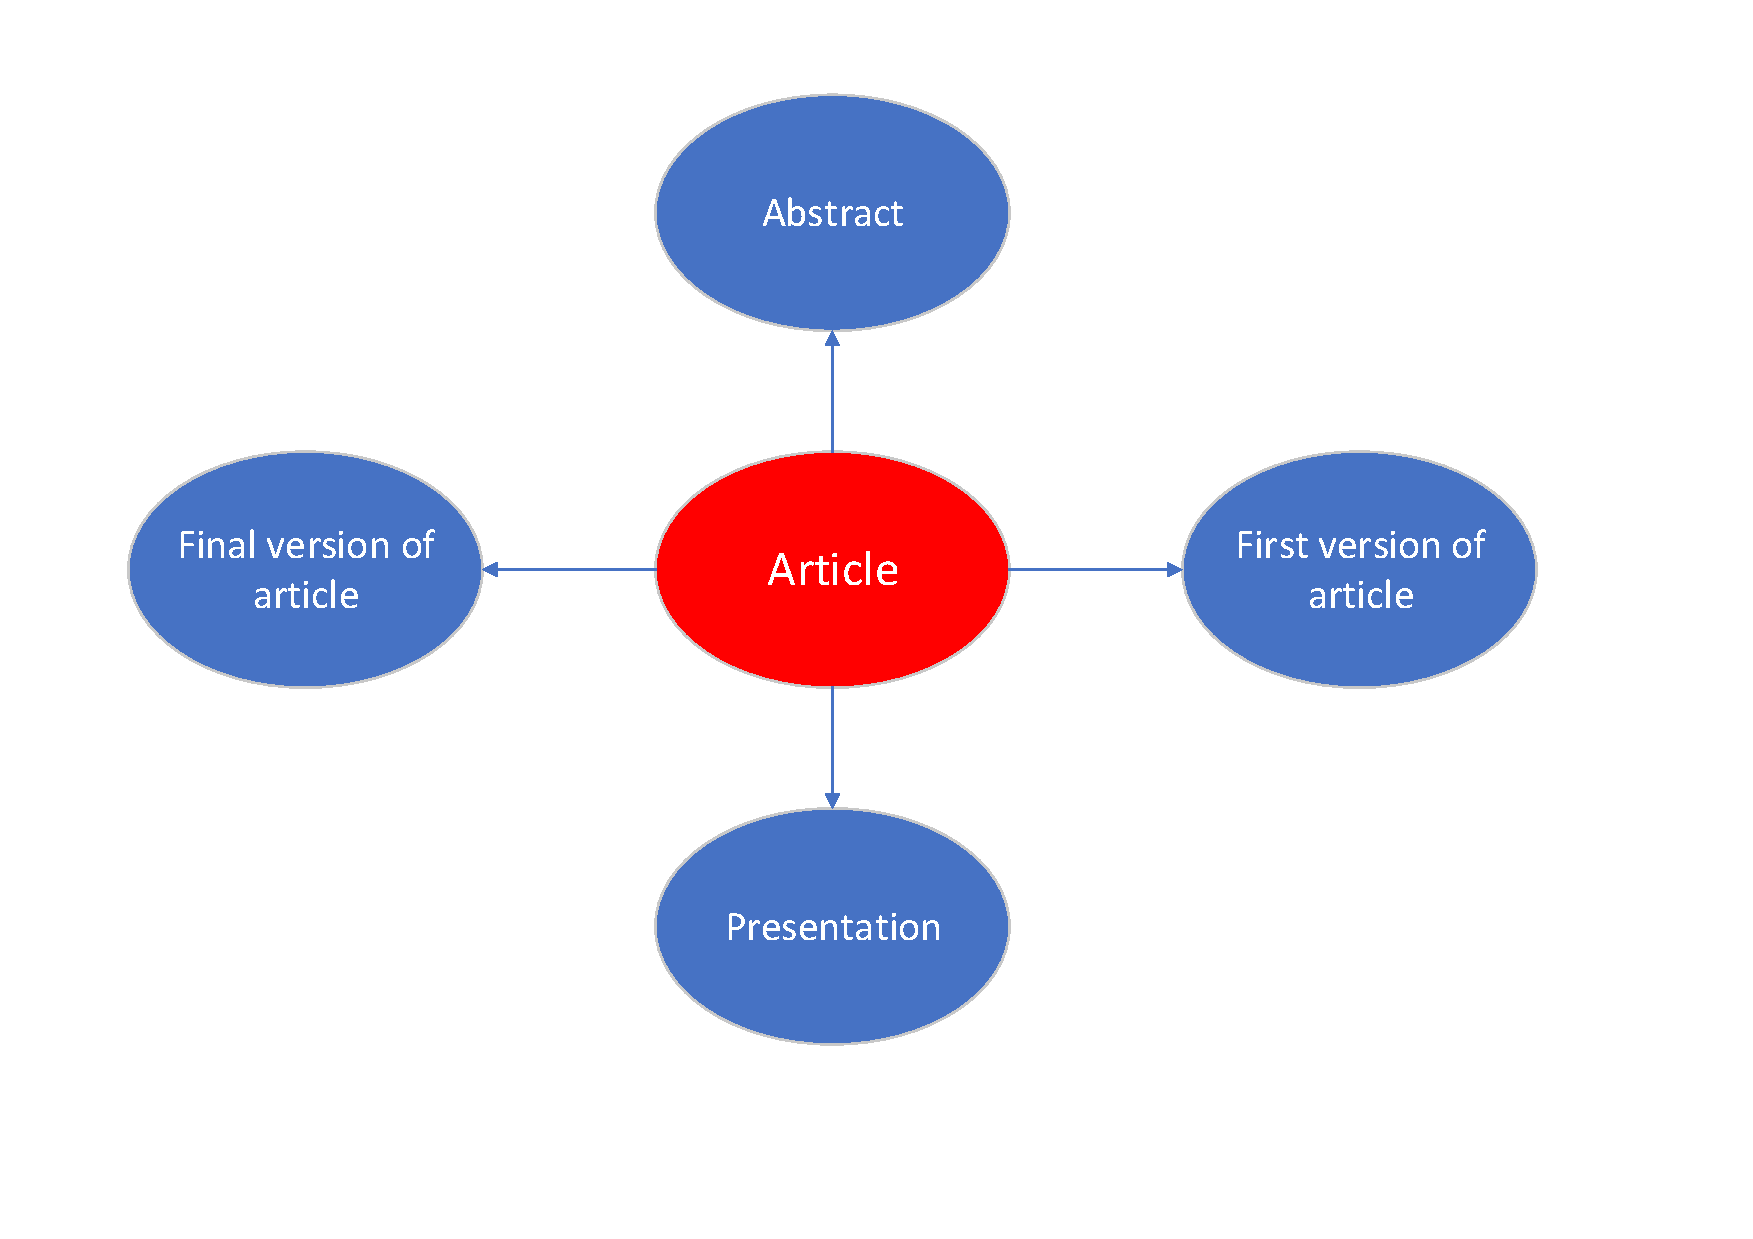
\includegraphics[width=\textwidth]{Kresba}
\end{table}



\section{Ešte dôležitejšia časť} \label{dolezitejsia}
\begin{table} [hbtp]
    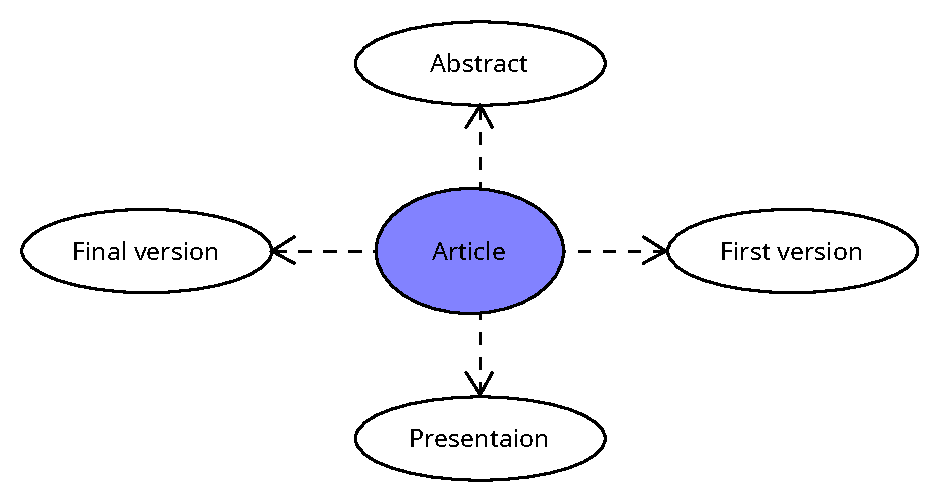
\includegraphics{Diagram}
\end{table}

\section{Najdôležitejšia časť} \label{najdolezitejsia}

Lorem ipsum dolor sit amet, consectetur adipiscing elit. Fusce blandit hendrerit enim, sit amet vestibulum quam egestas a. Nunc arcu magna, auctor a bibendum at, lobortis a tortor. Donec pretium malesuada leo, in pulvinar eros dictum quis. Vestibulum varius eros at vestibulum varius. Mauris ac sem euismod, elementum ex elementum, consectetur orci. In hac habitasse platea dictumst. Quisque maximus justo finibus, egestas eros eu, rutrum quam. Fusce at felis congue, interdum enim non, pretium arcu. Duis mi ex, dapibus sed mi dapibus, lobortis tempor mi. Praesent cursus ipsum sit amet ante ultrices, id posuere metus fringilla. Integer sollicitudin aliquet nulla, id consectetur metus tincidunt a. Proin sagittis ante a nisl interdum venenatis. Aliquam lacinia efficitur metus, sit amet malesuada mauris. Maecenas gravida a lacus nec hendrerit. Aenean porttitor, lacus et sollicitudin consectetur, ipsum odio luctus libero, non rutrum nibh sapien blandit ligula. Proin diam ipsum, molestie quis dignissim quis, gravida eget justo.


\section{Záver} \label{zaver} % prípadne iný variant názvu



%\acknowledgement{Ak niekomu chcete poďakovať\ldots}


% týmto sa generuje zoznam literatúry z obsahu súboru literatura.bib podľa toho, na čo sa v článku odkazujete
\bibliography{literatura}
\bibliographystyle{abbrv} % prípadne alpha, abbrv alebo hociktorý iný
\end{document}
